\documentclass[journal]{IEEEtran}
%\hyphenation{op-tical net-works semi-conduc-tor}

\usepackage{graphicx}
\usepackage{caption}
\usepackage{subcaption}
\usepackage{amsmath}
\usepackage{bm}
\usepackage{balance}

\usepackage{color}
\definecolor{cite_col}{rgb}{0.5,0,0}
\definecolor{link_col}{rgb}{0,0.5,0}
\definecolor{url_col}{rgb}{0,0,0.5}
\usepackage[pdftex,breaklinks=true,colorlinks=true,citecolor=cite_col,linkcolor=link_col,urlcolor=url_col,bookmarks=true,bookmarksopen=true]{hyperref}

\usepackage{balance}
\usepackage{pdfpages}
\usepackage{refcount}
\usepackage{bookmark}
\makeatletter
\define@key{pdfpages}{linkname}{\def\AM@linkname@option{#1}\label{pdfpages@#1@begin}}
\newcommand*{\mypdfbookmark}[4]{\bookmark[page=\numexpr\getpagerefnumber{pdfpages@#1@begin}+#2\relax,view={#3}]{#4}}
\makeatother

\begin{document}
\title{Robust Optical Flow in low SNR Thermal-Infrared}

\author{Stephen~Vidas,~\IEEEmembership{Member,~IEEE,}
        Vu~Hoang~Minh,~\IEEEmembership{Member?,~IEEE,}
        and~C.C.~Cheah,~\IEEEmembership{Senior~Member?,~IEEE}% <-this % stops a space
\thanks{All authors are with the School of Electrical and Electronic Engineering,
Nanyang Technological University, Singapore, 639798
e-mail: hoangmin001@e.ntu.edu.sg,\{svidas,ecccheah\}@ntu.edu.sg.}% <-this % stops a space
}

\markboth{Journal TBA}%
{Journal TBA}
% The only time the second header will appear is for the odd numbered pages
% after the title page when using the twoside option.
%
% *** Note that you probably will NOT want to include the author's ***
% *** name in the headers of peer review papers.                   ***
% You can use \ifCLASSOPTIONpeerreview for conditional compilation here if
% you desire.

\maketitle

% As a general rule, do not put math, special symbols or citations
% in the abstract or keywords.
\begin{abstract}
...
\end{abstract}

% Note that keywords are not normally used for peerreview papers.
%\begin{IEEEkeywords}
%IEEEtran, journal, \LaTeX, paper, template.
%\end{IEEEkeywords}

% For peerreview papers, this IEEEtran command inserts a page break and
% creates the second title. It will be ignored for other modes.
\IEEEpeerreviewmaketitle

% INTRODUCTION
\section{Introduction}
\label{sec:introduction}
[Motivation] 
Thermal-infrared imaging has been proven to have advantageous properties in difficult lighting conditions such as darkness, dust, smoke and fog; especially for the tasks of detecting humans, animals, powered equipment and other anomalies. Because of this, a thermal-infrared camera is already an appealing choice to be part of a robot- or human-mounted sensor configuration for modern search and rescue, firefighting or exploration tasks. However,more can be done with the thermal-infrared video than simply 2D visualization and detection, in that it is possible to implement a SLAM (Simultaneous Localization And Mapping) system to enable a 3D understanding of the environment, including the position of the human or robot within it. This information is crucial for navigation purposes, as well as planning purposes for emergency response.

[Applications]
Firefighting \cite{Schonauer}, Search \& Rescue [?], Robot navigation \cite{Maddern, Gonzalez2011}, Energy auditing [cite Steve's journal paper if it's published in time] and Exploration [?].

Examples of some recent investigations into these areas (can we find relevant citations for these kinds of work?)
\begin{itemize}
	\item 3D "Building Reconstruction and Thermal Mapping in Fire Brigade Operations Categories and Subject Descriptors" \cite{schonauer20133d}. Link 
	http://www.youtube.com/watch?v=QtNvHBT3jMs   	 
	\item http://youtu.be/BB8jojwl7ws?t=6m30s
\end{itemize}

[Contributions]
These are what we are aiming for, for this initial paper:
\begin{itemize}
	\item Continuous real-time operation on a standard PC (at least 10 frames per second, aiming more for 30)
	\item Appropriate default parameters (or adaptive parameters) for a range of typical and atypical environments and data sequences
	\item Tracking that can maintain a large number of stable and well-distributed features under the following challenges:
		\begin{itemize}
			\item sudden movements
			\item forwards and backwards motion
			\item fairly low SNR
		\end{itemize}
	\item Well-documented, cross-platform, OpenCV/C++ based library, integrated with ROS, that can be used for sparse optical flow on thermal-infrared
\end{itemize}

[Structure]

\begin{itemize}
	\item motivation
	\item contributions
	\item intro to structure
\end{itemize}

Placeholder citation \cite{Vidas2011}.

% BACKGROUND
\section{Background}
\label{sec:background}
Placeholder Figure \ref{fig:dummy}.

\begin{figure}
\centering

\includegraphics[width=1.0\columnwidth]{media/dummy.jpg}
\caption{...}
\label{fig:dummy}
\end{figure}


\subsection{Thermal-Infrared Computer Vision}
\label{sec:background_thermal}
Some information on calibration \cite{Vidas2012a}.

NUCs and other useful information for researchers to get stuck into solving similar problems with thermal-IR cameras.
A lot of this can be sourced from Steve's thesis (especially Chapter 2).


\subsection{Sparse Optical Flow}
\label{sec:background_sparse_of}
...

% RELATED WORK
\section{Related Work}
\label{sec:related_work}
\input{sources/related_work.tex}

\subsection{Image Denoising}
\label{sec:related_work_denoising}
\cite{Buades}, \cite{Hou2011}, \cite{dabov2007image}

\subsection{Feature Detection}
\label{sec:related_work_feature_detection}
\cite{Vidas2011}, \cite{Yung2008}

\subsection{Feature Tracking}
\label{sec:related_work_feature_tracking}
\cite{Vidas2012}

Can include some references to paper/s on object tracking in thermal-ir, with disclaimer that by tracking living or powered things like people or vehicles, the images are by definition high SNR, so the problem is much easier

% METHOD
\section{Proposed Method}
\label{sec:method}
Aims:

\begin{itemize}
	\item enable detection and tracking of features in low SNR regions
	\item ensure a good distribution of tracked features
	\item default values should perform well for all kinds of thermal images
\end{itemize}

Flowchart, Figure \ref{fig:optical_flow_flowchart}.

\begin{figure}
\centering
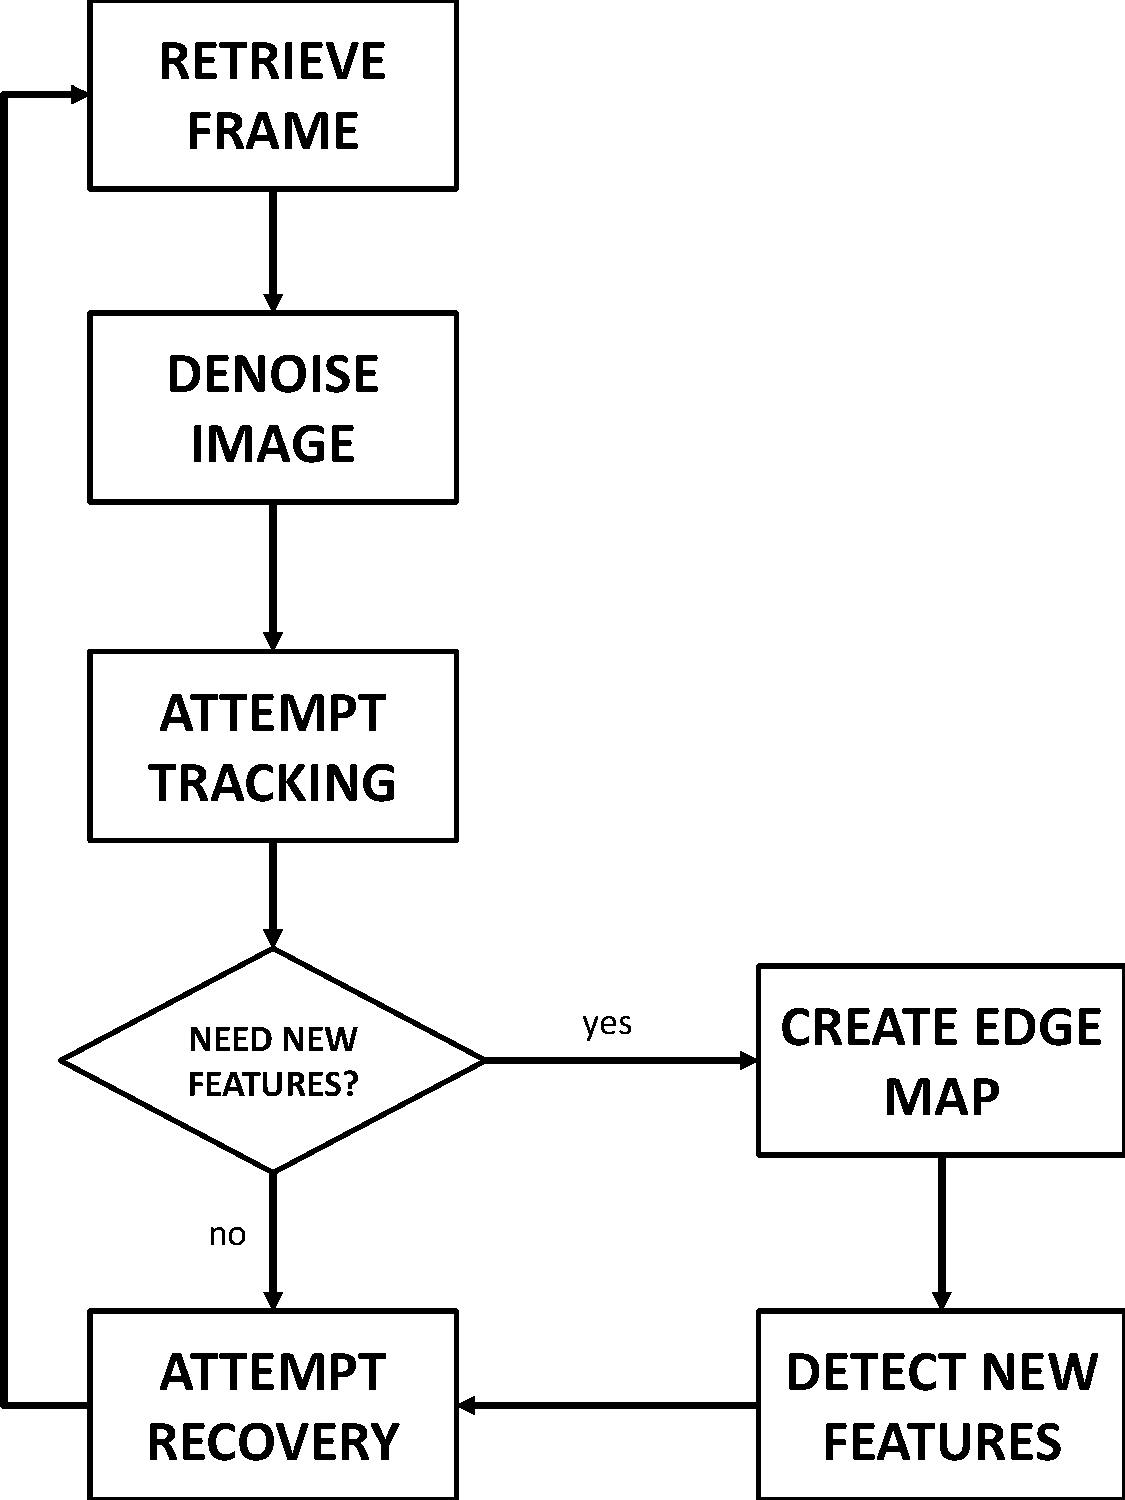
\includegraphics[width=1.0\columnwidth]{media/optical_flow_flowchart.pdf}
\caption{Flow chart demonstrating high-level optical flow procedure.}
\label{fig:optical_flow_flowchart}
\end{figure}



\subsection{Feature Tracking}
\label{sec:method_feature_tracking}
Some contributions that were not included in previous paper:

\begin{itemize}
	\item LDA-based matching for interruption handling
	\item initial warp for minimizing search windows based on feature velocity
	\item adaptive tracking window, based on no. of features and feature velocity:
	\begin{itemize}
	  \item this appropriately limits the spatial size of the search space for each new projection in order to reduce processing time while simultaneously decrease chance of incorrect tracking, without preventing good tracking results
		\item no. of features relative to maximum and predefined frac defines maximum distance
		\item 2 times the expected required distance defines the minimum (well, 3 is the actual minimum)
	\end{itemize}
	\item scalable feature track management method enabling loop closure
	\begin{itemize}
	  \item limits memory consumption to a fixed, finite upper limit
		\item still provides opportunity to recover lost features and potentially enables loop closure
	\end{itemize}
\end{itemize}






% EXPERIMENTS
\section{Experiments}
\label{sec:experiments}
Timing tests were performed on a Intel Core I5-3317 CPU 1.7GHz, 8GB RAM. 

Experiments have been designed to assess the effectiveness of the proposed method compared to existing alternatives, as well as determine which aspects of the method have the most positive effect, and at what cost (in terms of processing time). 
(Each part of the evaluation will include FAST and/or other conventional methods as a baseline).

First, a new set of data sequences captured for the experiments is presented in Subsection \ref{sec:experiments_datasets}.
Second, the evaluation framework for the subsequent three subsections is defined in Subsection \ref{sec:experiments_framework}.
Third, several alternative denoising methods are compared for front-end image processing, and evaluated using both the proposed and conventional methods in Subsection \ref{sec:experiments_image_processing}.
Fourth, the edge detection and processing stage is evaluated in terms of performance and processing time in Subsection \ref{sec:experiments_edge_d_and_p}.
Fifth, the corner selection procedure based on the edge map is evaluated in Subsection \ref{sec:experiments_corner_selection}.
Sixth, tracking improvements are demonstrated in Subsection \ref{sec:experiments_tracking_improvements}.
Finally, the proposed method is evaluated on the same dataset as used by \cite{Vidas2012}, allowing a direct comparison with the best known past performance of a thermal-infrared sparse optical flow system in Subsection \ref{sec:experiments_me_stability}.

\subsection{Datasets}
\label{sec:experiments_datasets}
The evaluation is done on thermal images
collected and labeled by thermographic camera, Optris PI450, equipped with 80Hz
measurement speed and 382 x 288 pixels optical resolution \footnote{http://www.optris.com/thermal-imager-pi400}. With high speed capturing ability, Optris PI450 is sufficient for real-time application, namely Simultaneous Localization and Mapping (SLAM).   

Four datasets with different signal-to-noise (SNR) ratios  are used as follows. 
\begin{itemize}
\item High SNR indoor
\item Low SNR indoor 
\item High SNR outdoor
\item Low SNR outdoor 
\end{itemize}

Thermal images not in our database can be easily added to the training set without affecting any algorithms.








%A significant amount of
%noise is added during the acquisition process (zoom,
%viewpoint, light changes, Jpeg compression). The zoom
%changes involve a change in pixel intensity as automatic
%camera settings are used. Jpeg compression additionally
%introduces artifacts. Some of the image pairs are
%displayed in Section 5.2. In order to use a homography
%for verification we used planar scenes or 3D scenes
%with a fixed camera position. The homography between
%images was estimated using manually selected corresponding
%points. Each scale change sequence consists
%of scaled and rotated images, for which the scale factor
%varies from 1.4 to 4.5. For the viewpoint change
%sequences the viewpoint varies in the horizontal direction
%between 0 and 70 degrees. There are 10 images in
%each sequence representing different scenes. The experiments
%were carried out using 10 scale change sequences
%and 6 viewpoint change sequences of real images,
%one of the sequences is displayed in Fig. 9. There are 
%160 images in total and approximately 100 000 interest
%points are detected in these images and used to
%evaluate the detectors.


%Label and describe each of the datasets captured, with justification (e.g. for the variety).

%Figure \ref{fig:datasets} shows samples of datasets:

%\begin{figure}
%\centering
%	\begin{subfigure}{0.49\columnwidth}
%    \centering
%    
\includegraphics[width=1.00\textwidth]{media/dummy.jpg}
%    \caption{Sequence 1}
%		\label{fig:datasets_1}
%  \end{subfigure}
%	\begin{subfigure}{0.49\columnwidth}
%    \centering
%    
\includegraphics[width=1.00\textwidth]{media/dummy.jpg}
%		\caption{Sequence 2}
%		\label{fig:datasets_2}
%  \end{subfigure} \vspace{10pt} \\ 
%	\begin{subfigure}{0.49\columnwidth}
%    \centering
%    
\includegraphics[width=1.00\textwidth]{media/dummy.jpg}
%    \caption{Sequence 3}
%		\label{fig:datasets_3}
%  \end{subfigure}
%	\begin{subfigure}{0.49\columnwidth}
%    \centering
%    
\includegraphics[width=1.00\textwidth]{media/dummy.jpg}
%		\caption{Sequence 4}
%		\label{fig:datasets_4}
%  \end{subfigure} \vspace{10pt} \\ 
%	\begin{subfigure}{0.49\columnwidth}
%    \centering
%    
\includegraphics[width=1.00\textwidth]{media/dummy.jpg}
%    \caption{Sequence 5}
%		\label{fig:datasets_5}
%  \end{subfigure}
%	\begin{subfigure}{0.49\columnwidth}
%    \centering
%    
\includegraphics[width=1.00\textwidth]{media/dummy.jpg}
%		\caption{Sequence 6}
%		\label{fig:datasets_6}
%  \end{subfigure} \vspace{10pt} \\ 
%	\begin{subfigure}{0.49\columnwidth}
%    \centering
%    
\includegraphics[width=1.00\textwidth]{media/dummy.jpg}
%    \caption{Sequence 7}
%		\label{fig:datasets_7}
%  \end{subfigure}
%	\begin{subfigure}{0.49\columnwidth}
%    \centering
%    
\includegraphics[width=1.00\textwidth]{media/dummy.jpg}
%		\caption{Sequence 8}
%		\label{fig:datasets_8}
%  \end{subfigure}
%\caption{Datasets for evaluation}
%\label{fig:datasets}
%\end{figure}

\subsection{Framework}
\label{sec:experiments_framework}
This is where you explain the basic experiments you will be doing. When it comes to judging the performance of the feature detection algorithms (and implicitly, the image processing algorithms), I recommend emphasizing the following characteristics:

\begin{itemize}
	\item trackability - looking at for example the average lifetime of detected features, and how far they "`drift"' throughout the sequence. Can use my reversal technique here (looping from 0 to 100 and back to 0 without doubling up, and comparing the start and end location of the tracked feature)
	\item precision - how accurately the features are detected on valid points-of-interest, as reflected in the repeatability of detections (whether the exact same points are detected in the real world even when the camera has shifted to a different view). You can compare each new detection with how the features have been tracked using Lucas-Kanade, but this will probably also require manual (human) verification.
	\item quality assessment - looking at how effective the feature ranking (strength metrics) are. You can probably use some qualitative analysis here, with some good figures, but also you can consider looking at the relationship between feature quality, and other parameters such as the precision and trackability of the feature, to determine how well the quality metric works.
\end{itemize}

You should show some comparative images from FAST and the proposed detector (perhaps with a low SNR and high SNR image each) which show the top N features from each detector. The top N from the proposed detector should seem much more logical/intuitive. Later experiments will demonstrate a good relationship between the feature "`strength"' and its usefulness/effectiveness.

The framework should make clear that you want to investigate changing parameters such as:

\begin{itemize}
	\item denoising method
	\item feature detection method
	\item feature ranking/sorting method
	\item thresholds and sensitivity levels
\end{itemize}

\subsection{Image Processing}
\label{sec:experiments_image_processing}
%This section should be where you establish the effectiveness of the two denoising methods, including their processing time, by using existing (conventional) feature detectors such as FAST and HARRIS, and a conventional tracking algorithm such as Lucas-Kanade. 
%You should also include your own proposed method in the evaluation.
%
%Also, you should look at the effect of different methods of scaling the 14-bit data to 8-bit format. The advantage of 8-bit format is that it requires less processing time, and also allows more modularity with existing functions and libraries. Furthermore, there should generally be very little (if any) information lost in this conversion, and when information is lost, it means it is a high SNR image and so the loss of the information is not a problem (there is still sufficient information left over).



%We propose a novel image denoising strategy based on an enhanced sparse representation in transform domain. The enhancement of the sparsity is achieved by grouping similar 2D image fragments (e.g., blocks) into 3D data arrays which we call "groups." Collaborative Altering is a special procedure developed to deal with these 3D groups. We realize it using the three successive steps: 3D transformation of a group, shrinkage of the transform spectrum, and inverse 3D transformation. 
%The result is a 3D estimate that consists of the jointly filtered grouped image blocks. By attenuating the noise, the collaborative filtering reveals even the finest details shared by grouped blocks and, at the same time, it preserves the essential unique features of each individual block. The filtered blocks are then returned to their original positions. Because these blocks are overlapping, for each pixel, we obtain many different estimates which need to be combined. Aggregation is a particular averaging procedure which is exploited to take advantage of this redundancy. A significant improvement is obtained by a specially developed collaborative Wiener filtering

In this section, authors would like to establish the effectiveness of the two proposed denoising methods, namely Non-local algorithm \cite{Buades} and Transform-domain collaborative filtering \cite{dabov2007image}. In short, first method analyzes noise for  local smoothing filters followed by computing nonlocal means whilst second approach groups 2D image fragments into 3D data arrays to unveil the finest details based on aggregation and collaborative Wiener filtering.  

Compare to Transform-domain collaborative filtering in terms of processing time, Non-local means is about 5 time faster. However, in terms of output quality, Transform-domain collaborative filtering is incomparable and still state-of-the-art method for denoising target. As a result, we propose to employ first denoising technique in case of low noise level. Otherwise, second approach is used to ameliorate further-processing steps. To classify whether an image is noisy or not, we profound applying an estimation of noise level based on Bayesian MAP inference \cite{liu2006noise} and analogizing to a predefined threshold of 5 (for 0-255 grayscale) (need to find this threshold!?).

To evaluate the effectiveness of two proposed denoising methods, two thermal images with different level of SNR are introduced. Next, feature detectors, namely FAST \cite{rosten2006machine} and HARRIS \cite{harris1988combined}, are deployed in noisy and denoised frames for collation. The  minimum accepted quality of corners and minimum intensity parameters \footnote{http://www.mathworks.com/help/vision/ref/detectfastfeatures.html}, are set at 0.005 in both methods and 0.05 in FAST, respectively.  The results are shown in Fig. \ref{fig:imgprocessing}.

\begin{figure}
\centering
	\begin{subfigure}{0.49\columnwidth}
    \centering
    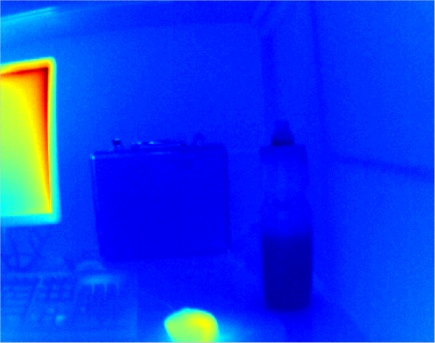
\includegraphics[width=1.00\textwidth]{media/V_C_highsnr.jpg}
	    \caption{}
		\label{fig:imgprocessing_1}
  \end{subfigure}
	\begin{subfigure}{0.49\columnwidth}
    \centering
    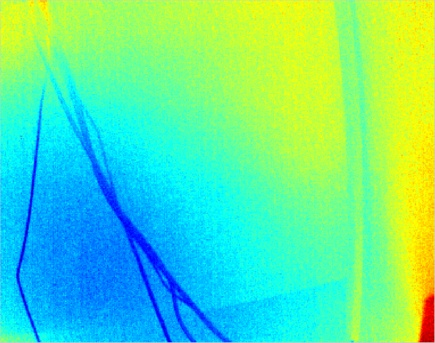
\includegraphics[width=1.00\textwidth]{media/V_C_lowsnr.jpg}
		\caption{}
		\label{fig:imgprocessing_2}
  \end{subfigure} \vspace{10pt} \\ 
	\begin{subfigure}{0.49\columnwidth}
    \centering
    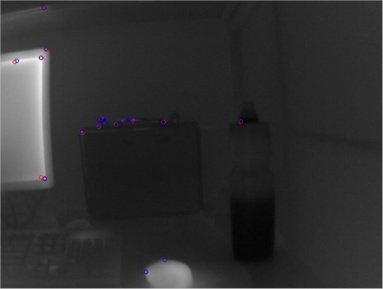
\includegraphics[width=1.00\textwidth]{media/V_C_highsnrcornersori.jpg}
    	\caption{}
		\label{fig:imgprocessing_3}
  \end{subfigure}
	\begin{subfigure}{0.49\columnwidth}
    \centering
    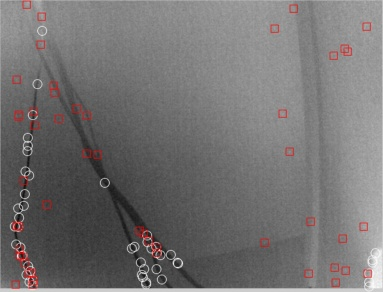
\includegraphics[width=1.00\textwidth]{media/V_C_lowsnrcornersori.jpg}
		\caption{}
		\label{fig:imgprocessing_4}
  \end{subfigure} \vspace{10pt} \\ 
	\begin{subfigure}{0.49\columnwidth}
    \centering
    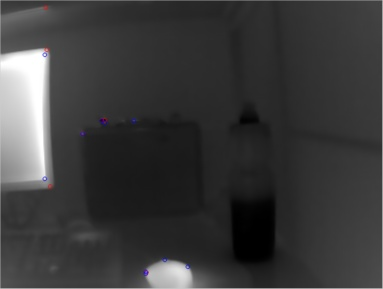
\includegraphics[width=1.00\textwidth]{media/V_C_highsnrcornersnonlocal.jpg}
    	\caption{}
		\label{fig:imgprocessing_5}
  \end{subfigure}
	\begin{subfigure}{0.49\columnwidth}
    \centering
    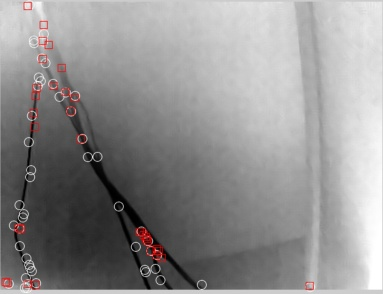
\includegraphics[width=1.00\textwidth]{media/V_C_lowsnrcornersnonlocal.jpg}
		\caption{}
		\label{fig:imgprocessing_6}
  \end{subfigure} \vspace{10pt} \\ 
	\begin{subfigure}{0.49\columnwidth}
    \centering
    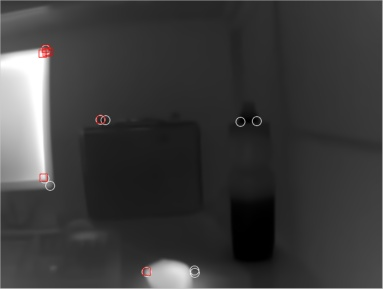
\includegraphics[width=1.00\textwidth]{media/V_C_highsnrcornerstrans.jpg}
    	\caption{}
		\label{fig:imgprocessing_7}
  \end{subfigure}
	\begin{subfigure}{0.49\columnwidth}
    \centering
    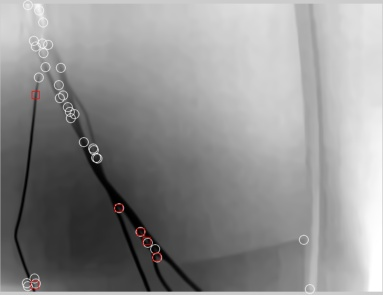
\includegraphics[width=1.00\textwidth]{media/V_C_lowsnrcornerstrans.jpg}
		\caption{}
		\label{fig:imgprocessing_8}
  \end{subfigure}
\caption{Image processing evaluation: (a,b) original high and low SNR frames, (c,d) gray-scale frames, (e,f) non-local means denoised frames, (g,h)  transform-domain collaborative filtering denoised frames, white circles and red rectangular denote feature points by Harris and FAST methods, respectively}
\label{fig:imgprocessing}
\end{figure}

%MinQuality 0.005 - both
%MinContrast 0.05 - Fast
%corners1 = detectHarrisFeatures(grayImage,'MinQuality',0.005);
%corners2=detectFASTFeatures(grayImage,'MinQuality',0.005,'MinContrast',0.05);
%A=corners1.selectStrongest(50).Location;
%B=corners2.selectStrongest(50).Location;
%figure;imshow(grayImage);axis off;hold on
%scatter(A(:,1),A(:,2),50,'w');
%scatter(B(:,1),B(:,2),50,'r','s');
%export_fig V_C_lowsnrcornersori.jpg


%In high SNR thermal images, such as Fig. \ref{fig:imgprocessing_1}, both denoising methods output 


\subsection{Edge Detection and Processing}
\label{sec:experiments_edge_d_and_p}
%This is where you will assess the effectiveness of different thresholds and/or settings for the edge detection, and also establish which (if any) of your proposed filters and other methods actually improve performance, and how fast they are.




In this section, the effectiveness 



authors would like to establish the effectiveness of the two proposed denoising methods, namely Non-local algorithm \cite{Buades} and Transform-domain collaborative filtering \cite{dabov2007image}. In short, first method analyzes noise for  local smoothing filters followed by computing nonlocal means whilst second approach groups 2D image fragments into 3D data arrays to unveil the finest details based on aggregation and collaborative Wiener filtering.  


\subsection{Corner Selection}
\label{sec:experiments_corner_selection}
This section should be where you establish the effectiveness of the two denoising methods, including their processing time, by using existing (conventional) feature detectors such as FAST and HARRIS, and a conventional tracking algorithm such as Lucas-Kanade.

Also, you should look at the effect of different methods of scaling the 14-bit data to 8-bit format. The advantage of 8-bit format is that it requires less processing time, and also allows more modularity with existing functions and libraries. Furthermore, there should generally be very little (if any) information lost in this conversion, and when information is lost, it means it is a high SNR image and so the loss of the information is not a problem (there is still sufficient information left over).

\subsection{Tracking Improvements}
\label{sec:experiments_tracking_improvements}
Want to demonstrate the following:

\begin{itemize}
	\item adaptive windows can reduce processing time without sacrificing performance, and simultaneously reduce chance of incorrect matching
	\item scalable feature track management method limits memory consumption, prevents lagging, maintains ability to recover lost features
\end{itemize}

\subsection{Motion Estimation Stability}
\label{sec:experiments_me_stability}
Gain access to the exact same sequences used by Steve for his previous paper. 
Run the 3D motion estimation / monocular SLAM system (when ready) on these sequences, using your proposed methods. 
Superimpose results on the same plot as used in the previous paper, to show that error has been much improved.

Mean time until failure can be defined as the metric.

% CONCLUSION
\section{Conclusion}
\label{sec:conclusion}
...

\section*{Acknowledgment}

(Will need to check if this is necessary with Prof Cheah)
The authors would like to thank the funding from A*STAR, Singapore's National Research funding agency, for the support of this project.

\bibliographystyle{myIEEEtran}
\bibliography{mypapers}

\end{document}
